\section{What we explored and learned}
\label{sec:journey}

The pipeline of Section~\ref{sec:method} is the result of two attempts, several failures and a few measurements that changed our plans (Figure~\ref{fig:journey}). This section follows them in order, because most of what we learned came from them.

\begin{figure}[!htb]
\centering
\begin{adjustbox}{max width=\linewidth}
\begin{tikzpicture}[
  node distance=2.5mm and 4mm,
  every node/.style={font=\footnotesize\setstretch{1}},
  phase/.style={draw, rounded corners, fill=blue!8, text width=4.4cm, align=center, minimum height=14.5mm},
  note/.style={draw, dashed, fill=gray!7, text width=7.6cm, align=left, minimum height=14.5mm},
  bad/.style={draw, rounded corners, fill=red!10, text width=3.7cm, align=center, minimum height=12mm},
  good/.style={draw, rounded corners, fill=green!14, text width=3.7cm, align=center, minimum height=12mm},
  arr/.style={-{Stealth[length=2mm]}, thick},
  lnk/.style={densely dotted, thick, gray}]
\node[phase] (v1) {\textbf{v1} (Aug--Sep 2026)\\image poses, 6\,GB laptop};
\node[note, right=of v1] (n1) {Plain walls: COLMAP registered 24\% of the walk; a learned matcher had 49\,cm error and the model collapsed. Whole-room training peaked at 4k steps.};
\node[phase, below=of v1] (re) {\textbf{Restart as v2} (3 Oct)\\phone poses and depth};
\node[note, right=of re] (n2) {MuSHRoom first: phone data plus a laser scan to measure against. SuperSplat already walks, so no viewer of our own.};
\node[phase, below=of re] (g1) {\textbf{G0--G1} train \texttt{vr\_room}\\on a shared A100};
\node[note, right=of g1] (n3) {Out of memory with 1\,M seed points $\Rightarrow$ ``lite'' settings, checkpoints every 1k steps, automatic resume; three upstream bugs patched.};
\node[phase, below=of g1] (g2) {\textbf{G2} walk in SuperSplat};
\node[note, right=of g2] (n4) {Viewer froze on a missing setting; the PLY-to-viewer frame was measured, not assumed.};
\node[phase, below=of g2] (g3) {\textbf{G3} DN-Splatter vs plain splats};
\node[note, right=of g3] (n5) {Mesh 1.8 vs 5.9\,cm from the laser scan for 0.5\,dB less PSNR $\Rightarrow$ keep DN-Splatter.};
\node[phase, below=of g3] (g4) {\textbf{G4} our own room\\(iPhone 13 Pro, Polycam)};
\node[note, right=of g4] (n6) {Kaggle sessions lost at the 12\,h limit; frames saved sideways; floor found on the beds $\Rightarrow$ two alignment fixes.};
\node[phase, below=of g4] (g8) {\textbf{G8} find a novelty\\criteria fixed first};
\node[bad, below=6mm of g8.south, xshift=-2.0cm, anchor=north east] (a1) {\textbf{1. Capture check}\\coverage did not predict error $\times$};
\node[bad, right=4mm of a1] (a2) {\textbf{2. Tracking repair}\\nothing to repair $\times$};
\node[good, right=4mm of a2] (a3) {\textbf{3. Collision accuracy}\\3 of 4 criteria met; Polycam added};
\foreach \a/\b in {v1/re, re/g1, g1/g2, g2/g3, g3/g4, g4/g8} \draw[arr] (\a) -- (\b);
\foreach \a/\b in {v1/n1, re/n2, g1/n3, g2/n4, g3/n5, g4/n6} \draw[lnk] (\a) -- (\b);
\draw[arr] (g8.south) -- ++(0,-3mm) -| (a1.north);
\draw[arr] (g8.south) -- ++(0,-3mm) -| (a2.north);
\draw[arr] (g8.south) -- ++(0,-3mm) -| (a3.north);
\end{tikzpicture}
\end{adjustbox}
\caption{How the project developed. Blue: goals worked through in order; dashed: what each step taught us; red and green: the three novelty attempts and whether they met the criteria fixed before running them.}
\label{fig:journey}
\end{figure}

\subsection{v1: poses from images on a laptop}
Our first version aimed to reconstruct a room from RGB images alone and to train on a laptop (RTX~3050, 6\,GB). The test room was a plain-walled ARKitScenes \cite{baruch2021arkitscenes} bedroom (scene 41254269, a 95\,s iPad walk). Table~\ref{tab:v1poses} compares the pose sources we tried against the iPad's own ARKit poses. COLMAP \cite{schoenberger2016colmap} was accurate but registered only a quarter of the walk; SuperPoint \cite{detone2018superpoint} and LightGlue \cite{lindenberger2023lightglue} in hloc \cite{sarlin2019hloc} registered every frame with 49\,cm error, and 3DGS trained on those poses rendered every view as flat colour. A textured utility room, by contrast, tracked cleanly (COLMAP: all frames, 1.6\,cm). Image-only poses failed specifically on plain walls, and accuracy mattered more than coverage.

\begin{table}[!htb]
\caption{v1 pose sources on the plain-walled ARKitScenes bedroom 41254269 (laptop). Error is measured against the iPad's ARKit poses.}
\label{tab:v1poses}
\centering
\begin{tabular}{lccl}
\hline
\textbf{Pose source} & \textbf{Walk covered} & \textbf{Error} & \textbf{3DGS result} \\
\hline
COLMAP, SIFT & 24\% & 1.2\,cm & sharp, a quarter of the room \\
SuperPoint + LightGlue & 100\% & 49\,cm & total collapse \\
ORB-SLAM3 \cite{campos2021orbslam3}, mono & 7--93\% & 6--52\,cm & not trained (4--6 maps) \\
ARKit device poses & 100\% & reference & see Figure~\ref{fig:curves} \\
\hline
\end{tabular}
\end{table}

Even with ARKit poses, whole-room training did not hold: a 22\,s window of the walk reached 30.3\,dB on held-out frames, but the full walk peaked at 22.8\,dB after 4,000 steps and fell to 13.7\,dB by 15,000 (Figure~\ref{fig:curves}, left). Switching densification from MCMC \cite{kheradmand2024mcmc} to the default only slowed the decline, and we never found the cause. Only evaluating every 1,000 steps revealed the early peak; the final number alone said ``failure''. v1 also showed that its browser viewer, GaussianSplats3D \cite{gaussiansplats3d}, dropped to 8 frames per second (95th percentile) at a million Gaussians, and that a 32-photo phone capture made with NeRFCapture \cite{nerfcapture} trained to only 16.0\,dB, full of streaks and floaters.

\begin{figure}[!htb]
	\centering
	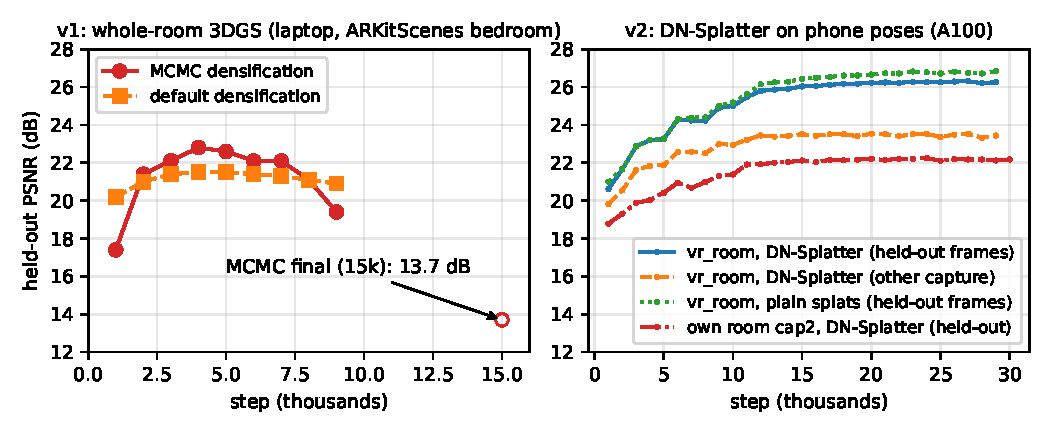
\includegraphics[width=\linewidth]{figures/curves.pdf}
	\caption{Held-out PSNR during training, evaluated every 1,000 steps. Left: v1, the full bedroom walk with ARKit poses on the laptop (from our v1 log; after 9k only the final value at 15k was recorded). Right: v2 on the A100: DN-Splatter on \texttt{vr\_room} (held-out frames of the training walk and frames of a separate walk), plain splats on the same data, and our own room. No v2 run collapsed.}
	\label{fig:curves}
\end{figure}

\subsection{Restarting as v2}
We kept the goal and changed the approach. The phone tracks its own pose by combining the camera with its inertial sensors, and those poses had trained a usable model where image-only poses had not, so v2 takes poses (and LiDAR depth) from the phone. DN-Splatter was chosen because it targets plain indoor surfaces and ships a loader for MuSHRoom, whose rooms come with iPhone data and a laser scan. SuperSplat already offered first-person walking with collision, so our plan to build a viewer in Unity was dropped. Training moved to a campus A100, and the work was organised as goals in priority order, each with exit criteria, so that unfinished goals could be cut from the end.

\subsection{Research code on a shared GPU}
Another user held 33--35\,GB of the A100's 40\,GB. DN-Splatter seeds one million Gaussians by default, and our first full run ran out of memory at about step 1,000. We changed as little as possible: 300k seed points, splitting stopped at step 10,000 instead of 15,000, and a wrapper that resumes from the newest checkpoint after a crash; a deliberate kill-and-resume test continued at step 1,001. Three upstream bugs had to be patched (an evaluation key error, a crash on resuming with an empty optimiser state, and resumed runs repeating their full step count), and the environment needed pins against conflicting dependency versions. Research code assumes a dedicated GPU and one uninterrupted run; checkpoints, regular evaluation and automatic resume are what made our runs finish.

\subsection{From a trained model to a walkable room}
A trained splat has no notion of up, floor, size or starting point. The viewer loads a PLY rotated by 180$^\circ$ about $z$, and its Euler-angle convention is undocumented; we measured both rather than assume them. The first walk test failed because our settings file lacked a block the viewer's newer schema requires. Our own room then broke two assumptions of our alignment. Polycam had saved every frame sideways, so the cameras' mean up vector averaged to almost nothing; up is now taken from the camera's $-x$ axis when $+y$ disagrees. The floor had been taken as the densest level below the cameras, which here was the tops of the beds, and the room came out 1.68 times too large; the floor is now the lowest dense level (Algorithm~\ref{alg:scene}). Against MuSHRoom's laser scan, the old rule had put the \texttt{vr\_room} floor 13\,cm too high and the new one is within about 1.5\,cm. The released \texttt{vr\_room} demo predates this fix and was deliberately kept as walk-tested.

\subsection{Capturing our own room}
Sejal captured a bedroom three times on an iPhone~13~Pro with Polycam's raw-data export \cite{polycam}. The first capture (32 frames) was too sparse, as v1 had predicted; the second (257 frames, one tracking segment) covered the room and was used; the third (491 frames) had three tracking segments with pose jumps of about 2\,m. While the A100 was full we tried Kaggle's free GPUs, but both sessions ran to Kaggle's 12-hour limit without saving output, most likely because our memory sampler outlived the training script (now stopped explicitly). Back on the A100, the run crashed once at step 10,400, resumed by itself from step 10,000 and finished.

\subsection{Looking for a novelty}
For each novelty idea we searched the literature first and fixed pass/fail criteria in writing before running anything. A capture check before training (Section~\ref{sec:capcheck-method}) failed its validation; a repair of \texttt{cap3}'s broken tracking found nothing to repair; the accuracy of walk collision met three of four criteria and is the result we lead with (Section~\ref{sec:results}).

The lessons that shaped the final design:
\begin{itemize}
\item take poses from the phone, since image-only poses failed on plain walls;
\item evaluate every 1,000 steps and look at renders, since a final number alone hid a collapse;
\item measure coordinate conventions and check alignment against a scan, since two of our assumptions were wrong on real data;
\item assume the GPU will run out: checkpoint, resume and keep evidence off the machine;
\item fix success criteria before the run and report the outcome either way.
\end{itemize}
